\documentclass[12pt]{article}

\newcommand{\Year}{2001}
\newcommand{\Ident}{GR0177}
\newcommand{\Version}{2.0}

\title{Solutions to \Year Physics GRE}
\author{Jonathan F. Dooley}

\usepackage{lipsum}
\usepackage{pdfpages}
\usepackage{setspace}
\usepackage{lineno} % linenumbers

% no indentation
\setlength{\parindent}{0pt}

\usepackage{graphicx, wrapfig, svg}
\usepackage[caption = false]{subfig}
\usepackage{caption}

\usepackage{color, colortbl}
\definecolor{lgray}{gray}{0.8}

\usepackage{newclude} % remove clearpage, include*

% allow \subsubsection and
\usepackage{titlesec}
\setcounter{secnumdepth}{4}
\setcounter{tocdepth}{4}

% create live links in TOC
\usepackage[hypertexnames=false]{hyperref}
\hypersetup{
  colorlinks = true,
  linkcolor = black,
  anchorcolor = black,
  citecolor = black,
  filecolor = black,
  urlcolor = black,
  pdfnewwindow = true,
  extension = pdf
}

\setlength{\parindent}{0pc}
\setlength{\parskip}{5pt plus1.5pt minus0.5pt} % <- from nmt thesis

\usepackage{lib/jfdgeom}
\usepackage{lib/jfdshorts}
\usepackage{lib/jfdtypeset}
\usepackage{lib/jfdcode}

\usepackage{pgre}
\usepackage{multicol}

\fancyfoot[C]{\thepage}
\fancyfoot[R]{\Ident\xspace Solutions v\Version}

\begin{document}
\TitlePage{\Year}{\Ident}{\Version}

\begin{center}
\boxed{\text{\large Q = Question \hspace{.2in} A = Answer \hspace{.2in}  P+ = Percent Correct in \Year }}
\end{center}
\begin{multicols}{5}
\begin{enumerate}
\item[Q] \begin{tabular}{cc} A & P+\end{tabular}
\item[Q] \begin{tabular}{cc} A & P+\end{tabular}
\item[Q] \begin{tabular}{cc} A & P+\end{tabular}
\item[Q] \begin{tabular}{cc} A & P+\end{tabular}
\item[Q] \begin{tabular}{cc} A & P+\end{tabular}
\end{enumerate}
\end{multicols}

\begin{multicols}{5}
\begin{enumerate}
\item[1] \begin{tabular}{cc} C & 54\%\end{tabular}
\item[2] \begin{tabular}{cc} D & 30\%\end{tabular}
\item[3] \begin{tabular}{cc} D & 71\%\end{tabular}
\item[4] \begin{tabular}{cc} C & 62\%\end{tabular}
\item[5] \begin{tabular}{cc} D & 28\%\end{tabular}
\item[]
\item[6] \begin{tabular}{cc} E & 34\%\end{tabular}
\item[7] \begin{tabular}{cc} B & 89\%\end{tabular}
\item[8] \begin{tabular}{cc} D & 65\%\end{tabular}
\item[9] \begin{tabular}{cc} A & 63\%\end{tabular}
\item[10] \begin{tabular}{cc} A & 53\%\end{tabular}
\item[]
\item[11] \begin{tabular}{cc} A & 28\%\end{tabular}
\item[12] \begin{tabular}{cc} E & 40\%\end{tabular}
\item[13] \begin{tabular}{cc} B & 42\%\end{tabular}
\item[14] \begin{tabular}{cc} C & 27\%\end{tabular}
\item[15] \begin{tabular}{cc} A & 68\%\end{tabular}
\item[]
\item[16] \begin{tabular}{cc} D & 14\%\end{tabular}
\item[17] \begin{tabular}{cc} B & 81\%\end{tabular}
\item[18] \begin{tabular}{cc} A & 45\%\end{tabular}
\item[19] \begin{tabular}{cc} B & 36\%\end{tabular}
\item[20] \begin{tabular}{cc} E & 49\%\end{tabular}

\item[]

\item[21] \begin{tabular}{cc} B & 60\%\end{tabular}
\item[22] \begin{tabular}{cc} A & 54\%\end{tabular}
\item[23] \begin{tabular}{cc} C & 45\%\end{tabular}
\item[24] \begin{tabular}{cc} C & 86\%\end{tabular}
\item[25] \begin{tabular}{cc} E & 49\%\end{tabular}
\item[]
\item[26] \begin{tabular}{cc} C & 30\%\end{tabular}
\item[27] \begin{tabular}{cc} A & 82\%\end{tabular}
\item[28] \begin{tabular}{cc} E & 61\%\end{tabular}
\item[29] \begin{tabular}{cc} C & 63\%\end{tabular}
\item[30] \begin{tabular}{cc} A & 44\%\end{tabular}
\item[]
\item[31] \begin{tabular}{cc} A & 53\%\end{tabular}
\item[32] \begin{tabular}{cc} D & 62\%\end{tabular}
\item[33] \begin{tabular}{cc} D & 31\%\end{tabular}
\item[34] \begin{tabular}{cc} C & 23\%\end{tabular}
\item[35] \begin{tabular}{cc} E & 82\%\end{tabular}
\item[]
\item[36] \begin{tabular}{cc} E & 70\%\end{tabular}
\item[37] \begin{tabular}{cc} D & 36\%\end{tabular}
\item[38] \begin{tabular}{cc} D & 35\%\end{tabular}
\item[39] \begin{tabular}{cc} D & 45\%\end{tabular}
\item[40] \begin{tabular}{cc} D & 40\%\end{tabular}

\item[]

\item[41] \begin{tabular}{cc} E & 66\%\end{tabular}
\item[42] \begin{tabular}{cc} C & 64\%\end{tabular}
\item[43] \begin{tabular}{cc} D & 39\%\end{tabular}
\item[44] \begin{tabular}{cc} D & 54\%\end{tabular}
\item[45] \begin{tabular}{cc} B & 50\%\end{tabular}
\item[]
\item[46] \begin{tabular}{cc} E & 29\%\end{tabular}
\item[47] \begin{tabular}{cc} B & 46\%\end{tabular}
\item[48] \begin{tabular}{cc} C & 57\%\end{tabular}
\item[49] \begin{tabular}{cc} E & 61\%\end{tabular}
\item[50] \begin{tabular}{cc} B & 50\%\end{tabular}
\item[]
\item[51] \begin{tabular}{cc} B & 45\%\end{tabular}
\item[52] \begin{tabular}{cc} C & 12\%\end{tabular}
\item[53] \begin{tabular}{cc} B & 32\%\end{tabular}
\item[54] \begin{tabular}{cc} C & 77\%\end{tabular}
\item[55] \begin{tabular}{cc} E & 62\%\end{tabular}
\item[]
\item[56] \begin{tabular}{cc} D & 54\%\end{tabular}
\item[57] \begin{tabular}{cc} A & 68\%\end{tabular}
\item[58] \begin{tabular}{cc} B & 58\%\end{tabular}
\item[59] \begin{tabular}{cc} B & 87\%\end{tabular}
\item[60] \begin{tabular}{cc} D & 55\%\end{tabular}

\item[]

\item[61] \begin{tabular}{cc} C & 18\%\end{tabular}
\item[62] \begin{tabular}{cc} A & 35\%\end{tabular}
\item[63] \begin{tabular}{cc} D & 52\%\end{tabular}
\item[64] \begin{tabular}{cc} A & 56\%\end{tabular}
\item[65] \begin{tabular}{cc} D & 44\%\end{tabular}
\item[]
\item[66] \begin{tabular}{cc} D & 33\%\end{tabular}
\item[67] \begin{tabular}{cc} E & 19\%\end{tabular}
\item[68] \begin{tabular}{cc} E & 51\%\end{tabular}
\item[69] \begin{tabular}{cc} B & 26\%\end{tabular}
\item[70] \begin{tabular}{cc} B & 53\%\end{tabular}
\item[]
\item[71] \begin{tabular}{cc} D & 32\%\end{tabular}
\item[72] \begin{tabular}{cc} E & 39\%\end{tabular}
\item[73] \begin{tabular}{cc} D & 43\%\end{tabular}
\item[74] \begin{tabular}{cc} D & 50\%\end{tabular}
\item[75] \begin{tabular}{cc} E & 57\%\end{tabular}
\item[]
\item[76] \begin{tabular}{cc} C & 49\%\end{tabular}
\item[77] \begin{tabular}{cc} E & 44\%\end{tabular}
\item[78] \begin{tabular}{cc} E & 52\%\end{tabular}
\item[79] \begin{tabular}{cc} D & 69\%\end{tabular}
\item[80] \begin{tabular}{cc} D & 28\%\end{tabular}

\item[]

\item[81] \begin{tabular}{cc} B & 50\%\end{tabular}
\item[82] \begin{tabular}{cc} D & 16\%\end{tabular}
\item[83] \begin{tabular}{cc} C & 30\%\end{tabular}
\item[84] \begin{tabular}{cc} D & 26\%\end{tabular}
\item[85] \begin{tabular}{cc} A & 25\%\end{tabular}
\item[]
\item[86] \begin{tabular}{cc} E & 24\%\end{tabular}
\item[87] \begin{tabular}{cc} A & 42\%\end{tabular}
\item[88] \begin{tabular}{cc} C & 42\%\end{tabular}
\item[89] \begin{tabular}{cc} E & 37\%\end{tabular}
\item[90] \begin{tabular}{cc} A & 33\%\end{tabular}
\item[]
\item[91] \begin{tabular}{cc} B & 41\%\end{tabular}
\item[92] \begin{tabular}{cc} E & 45\%\end{tabular}
\item[93] \begin{tabular}{cc} C & 42\%\end{tabular}
\item[94] \begin{tabular}{cc} E & 29\%\end{tabular}
\item[95] \begin{tabular}{cc} A & 42\%\end{tabular}
\item[]
\item[96] \begin{tabular}{cc} E & 13\%\end{tabular}
\item[97] \begin{tabular}{cc} E & 20\%\end{tabular}
\item[98] \begin{tabular}{cc} A & 72\%\end{tabular}
\item[99] \begin{tabular}{cc} D & 20\%\end{tabular}
\item[100] \begin{tabular}{cc} B & 72\%\end{tabular}

\item[]
\end{enumerate}
\end{multicols}
\clearpage

\Problem{1}{C}{%
The acceleration on the pendulum is the sum of the tangential and centripetal accelerations: $\vec{a} = \vec{a}_{tan} + \vec{a}_{cent}$ where

\begin{gather}
\vec{a}_{tan} = \frac{d\vec{v}}{dt} = \frac{d (\vec{\omega} r)}{d t} = r \frac{d\vec{w}}{dt} = r \vec{\alpha}\\
\vec{a}_{cent} = \frac{\vec{v}^{2}}{r} = \frac{\vec{\omega}^{2} r^{2}}{r} = \vec{\omega}^{2} r
\end{gather}
\\
At point $c$, $\vec{\omega} = const$ so the angular acceleration $\vec{\alpha} = \frac{d \vec{\omega}}{dt} = 0$. Therefore, $\vec{a} = \vec{a}_{cent}$. $\vec{a}_{cent}$ points towards the axis of rotation (pivot point), which eliminates (A), (B), and (D).\\
\\
At points $a$ and $e$, $\vec{\omega} = 0$ so that $\vec{a} = \vec{a}_{tan}$.
}

\Problem{2}{D}{%
This is a force balancing problem:

\begin{gather}
F_{cent} = F_{fr}\nonumber\\
m \hspace{.01in} \omega^{2} r = m g \mu_{s} \hspace{.1in} \rightarrow \hspace{.1in} r =\frac{g \mu_{s}}{\omega^2} \nonumber
\end{gather}
\\
for this equation to work we must correct the dimensions of $\omega$:

\begin{gather}
\omega= (33.3\Units{rev/min}) \left(   \frac{2 \pi\Units{rads}}{1\Units{rev}} \right)   \left(\frac{1\Units{min}}{60\Units{s}} \right) = 3.48\Units{rads/s}\nonumber\\
\nonumber\\
\therefore \hspace{.1in}r = \frac{10\Units{m s$^{-2}$} \cdot 0.30}{(3.48\Units{rad/s})^{2}} = 0.24\Units{m}\nonumber
\end{gather}
}


\Problem{3}{D}{%
Recall Kepler's Third Law:

\begin{gather}
T^{2} = \frac{4 \pi^{2} a^{3}}{G M}
\end{gather}
\\
where $T$ is the period, $a$ is the semi-major axis, M is the mass of the planet, and G is Newton's gravitational constant. For a circular orbit, both the semi-major and semi-minor axes are equal to $R$.

\begin{gather}
\therefore \hspace{.1in} T^{2} \propto R^{3} \hspace{.1in} \rightarrow \hspace{.1in} \boxed{T \propto R^{3/2}}\nonumber
\end{gather}
}

\Problem{4}{C}{%
From conservation of momentum, we can calculate the final velocity of the two particle system, $v_{f}$:

\begin{align}
p_{0} &= p_{f} \nonumber\\
2m v_{0} + 0 &= (2m + m) v_{f}\nonumber\\
\rightarrow \hspace{.1in} v_{f} &= \frac{2}{3} v_{0} \nonumber
\end{align}
\\
The fraction of initial kinetic energy lost in the collision can be found by dividing kinetic energy lost, $ T_{0} - T_{f} $, by the initial kinetic energy, $T_{0}$.

\begin{align}
\frac{T_{0} - T_{f}}{T_{0}} &=  \frac{   \frac{1}{2} (2m) v_{0}^{2} - \frac{1}{2} (3m) v_{f}^{2}   }{\frac{1}{2} (2m) v_{0}^{2}}\nonumber\\
&=\frac{ (2m) v_{0}^{2} - (3m) \left(  \frac{2}{3} v_{0} \right)^{2}   }{(2m) v_{0}^{2}}\nonumber\\
&= \frac{2 - \frac{12}{9} }{2} = \frac{\frac{18}{9} - \frac{12}{9}}{\frac{18}{9}} = \frac{6}{18} = \boxed{\frac{1}{3}}\nonumber
\end{align}
}

\Problem{5}{C}{%
The Equipartition Theorem states that

\begin{gather}
\langle  E  \rangle = \frac{f}{2} k_{B}T
\end{gather}
\\
Where $k_{B}$ is Boltzmann's constant, $T$ is the temperature, and $f$ is the degrees of freedom. The degrees of freedom for an oscillator in 1D, 2D, and 3D is found using the equation $f =$ (translational degrees) $+$ (rotational degrees) $+$ (vibrational degrees):\\

\hspace{2.7in}1D : $f = 2 + 0 + 0 = 2$

\hspace{2.7in}2D : $f = 2 + 1 + 1 = 4$

\hspace{2.7in}3D : $f = 3 + 2 + 1 = 6$\\
\\
Therefore, our three dimensional oscillator has average energy

\begin{gather}
\langle  E  \rangle = \frac{6}{2} k_{B}T = \boxed{ 3 k_{B} T  }\nonumber
\end{gather}
}

\Problem{6}{E}{%
Generally, in a closed cycle, an adiabatic process does less work than an isothermal process. To see this, note that on a PV diagram an isothermal expansion follows the curve $P \propto V^{-1}$ while an adiabatic expansion follows the curve $P \propto V^{-\gamma}$. Since $\gamma$ of an ideal monoatomic gas is greater then 1 ($\gamma = \frac{5}{3}$), the area under the isothermal curve (read: $W_{i}$) is greater then the area under the adiabatic curve ($W_{a}$). And both are greater than zero.

\begin{align}
\therefore \hspace{.1in} \boxed{0 < W_{a} < W_{i}}\nonumber
\end{align}
}

\Problem{7}{B}{%
Magnets with the same polarity repel one another. Therefore we can eliminate (A), (D), and (C).
\\\\
At small distances, the magnetic field lines are normal to the surface of the magnet and therefore we can eliminate (E) (Notice that (E) is the magnetic field produced by a current carrying wire, not two magnets).
}

\Problem{8}{D}{%
"A charge located above a grounded conduction plate" is almost always a method of images problem. Therefore we must picture an equal and opposite charge located a distance $L$ \textbf{below} the plate.
\\\\
The imagined charge is $-Q$. Therefore a net charge of $-Q$ is induced on the plate.
}


\Problem{9}{A}{%
Imagine a circle with an infinite number of charges of magnitude $q$ placed along its circumference. This is a model of a 2D hollow conductor which has an internal electric field equal to zero. Now remove all but 5 equally spaced charges. The symmetry of the system has the electric field vectors cancelling out with one another.
\\\\
Do not get tricked into adding up all five charges and choosing answer (C). This solution does not consider the symmetry and, therefore, the destructive superposition of the charges.
}


\Problem{10}{A}{%
The equivalent capacitance of capacitors in series and in parallel are

\begin{align}
\frac{1}{C_{eq}} = \frac{1}{C_{1}} + \frac{1}{C_{2}} + ... \hspace{.1in} \text{(Series)}\\
C_{eq} = C_{1} + C_{2} + ... \hspace{.1in} \text{(Parallel)}
\end{align}
\\
Therefore the equivalent capacitance of our capacitors is

\begin{align}
C_{eq} =\left(  \frac{1}{3\Units{\micro F}} + \frac{1}{6\Units{\micro F}}  \right)^{-1} = \frac{6\Units{\micro F}}{3\Units{\micro F}} = 2{\micro F} \nonumber
\end{align}
\\
The energy stored in a capacitor, $U$, is

\begin{gather}
U = \frac{1}{2} C_{eq} V^{2} =
\frac{1}{2} (2\e{-6}\Units{F}) (300\Units{V})^{2} =
\boxed{0.09\Units{J}}\nonumber
\end{gather}
}


\Problem{11}{A}{%
We must first find the location of the image produced by the 1st lens ($f_{1} = 20\Units{cm}$):

\begin{gather}
\label{eq:lens_pos} \frac{1}{f_{1}} = \frac{1}{s_{1}} + \frac{1}{s_{1}'}
\end{gather}

\begin{align}
\rightarrow \hspace{.1in} s_{1}' &= \left(   \frac{1}{20\Units{cm}} - \frac{1}{40\Units{cm}}  \right)^{-1} \nonumber\\
&= \left(   \frac{2}{40\Units{cm}} - \frac{1}{40\Units{cm}}  \right)^{-1} = 40\Units{cm}\nonumber
\end{align}
\\
The fact that $s_{1}'$ is a positive value tells us that the image is on the opposite side of the lens from the object (right side of lens). \\
\\
Now we look at the image produced by the 2nd lens. The object is no longer at $O$ but instead it is $s_{2} = 10\Units{cm}$ to the right of the 2nd lens (since it is $40\Units{cm}$ to the right of the 1st lens). By convention, this means that the equation for the image produced is

\begin{align}
\label{eq:lens_neg} \frac{1}{f_{2}} &= \frac{1}{s_{2}'} - \frac{1}{s_{2}}
\end{align}
\\
(Note the difference between equations \ref{eq:lens_pos} and  \ref{eq:lens_neg}) This is because the original object is to the right both lenses, so an object on the left would have a negative distance. We can now find the location of $s_{2}'$:

\begin{align}
\rightarrow \hspace{.1in} s_{2}' &= \left(   \frac{1}{f_{2}} + \frac{1}{s_{2}}   \right)^{-1}\nonumber\\
&= \left(   \frac{1}{10\Units{cm}} + \frac{1}{10\Units{cm}}   \right)^{-1} = \left(   \frac{2}{10\Units{cm}} \right)^{-1}  = 5\Units{cm}\nonumber
\end{align}
\\
Once again, because the produced image is positive, the location of the image is to the right of the lens.
\\\\
}


\Problem{12}{E}{%
The mirror equations states that

\begin{align}
\frac{1}{f} &= \frac{1}{s} + \frac{1}{s'}\\
\nonumber\\
\rightarrow  \hspace{.1in} \frac{1}{s'} &= \frac{1}{f}  - \frac{1}{s} \nonumber
\end{align}
\\
(same as \ref{eq:lens_pos}). Because $s < f$ we can conclude that $1/s > 1/f$. Therefore,

\begin{align}
\frac{1}{s'} &= \frac{1}{f}  - \frac{1}{s}  < 0\nonumber
\end{align}
\\
Which means that the image is not on the reflecting side of the mirror and must be at point $V$. This logic comes from the fact that, by convention, $s'$ is positive if produced on the same side as the object.
\\\\
}

\Problem{13}{B}{%
The angular separation of two point sources, $\theta$, is related to the the wavelength, $\lambda$, and telescope diameter, $D$ by the Rayleigh criterion:

\begin{gather}
D \sin{(\theta)} = 1.22 \lambda
\end{gather}
\\
Because $\theta$ is small be can approximate $\sin{(\theta)} \approx \theta$ (only true for \Units{rads}).\\
\\
We are asked to find the diameter needed for a telescope to resolve two stars with $\theta = 3\e{-5}\Units{rad}$  and $\lambda = 600\Units{nm}$. Plugging these values into the Rayleigh criterion and solving for $D$ we get

\begin{align}
D &= 1.22 \cdot \frac{ 600\Units{nm}}{ 3\e{-5}\Units{rad}}  = 1.22\cdot  \frac{6\e{-7}\Units{m}}{3\e{-5}\Units{rad}}\nonumber\\
\nonumber\\
&= 1.22\cdot 2\e{-2}\Units{m} = 2.44\e{-2}\Units{m} = 0.024\Units{m} \sim \boxed{2.5\Units{cm}}\nonumber
\end{align}
}


\Problem{14}{C}{%
This is a simple application of the point source illumination formula where $\sigma$ is the cross sectional area of the detector and $A$ is the area of the imagined sphere with $R = 1\Units{m}$

\begin{align}
I &= \frac{\sigma}{A} \\
\nonumber\\
&= \frac{\pi R^{2}} {4 \pi l^{2}} = \frac{R^{2}} {4 l^{2}} = \frac{(4\Units{cm})^{2}} {4 \cdot (100\Units{cm})^{2}} \nonumber\\
\nonumber\\
&= \frac{16}{4000} = \frac{4}{1000} = \boxed{4\e{-4}}\nonumber
\end{align}
}


\Problem{15}{A}{%
The most precise measurement could be incorrect, as long as the results of many measurements is very close the the average measurement. Therefore, the class that made the most precise measurement is the one with the smallest range of heights.
}

\Problem{16}{D}{%
A Poisson distribution describes radioactive phenomenon. In a poisson process the standard deviation, $\sigma$, can be found by taking the square root of the average, $\overline{x}$:

\begin{gather}
\overline{x} = \frac{3+0+2+1+2+4+0+1+2+5}{10} = \frac{20}{10} = 2\Units{counts/s}\nonumber\\
\nonumber\\
\therefore \hspace{.1in} \sigma = \sqrt{2} \nonumber
\end{gather}
\\
Now, the error on the mean is generally taken be to the standard deviation divided by the square root of the number of measurements, $N$:

\begin{gather}
\text{uncert} \hspace{.05in} = \frac {\sigma}{\sqrt{N}}
\end{gather}
\\
We need to find $N$ when the uncertainty is 1\% of the mean. \textbf{Be careful}  - do not set the uncertainty equal to $0.01$! Because the uncertainty is 1\% of the mean we need to use $0.01 \cdot \overline{x} = 0.02$:

\begin{gather}
0.02 = \frac {\sqrt{2}}{\sqrt{N}} \hspace{.1in} \rightarrow \hspace{.1in} 4\e{-4} = \frac{2}{N} \hspace{.1in} \rightarrow \hspace{.1in} N = \frac{2}{4\e{-4}} = \frac{1}{2\e{-4}} = 0.5\e{4} = \boxed{5000\Units{s}} \nonumber
\end{gather}
}


\Problem{17}{B}{%
The ground state means that each of the energy levels in the first few shells is filled by an electron (to the given maximum of 15 electrons). The electron configuration can be determined using the following diagram:

\begin{figure}[ht]
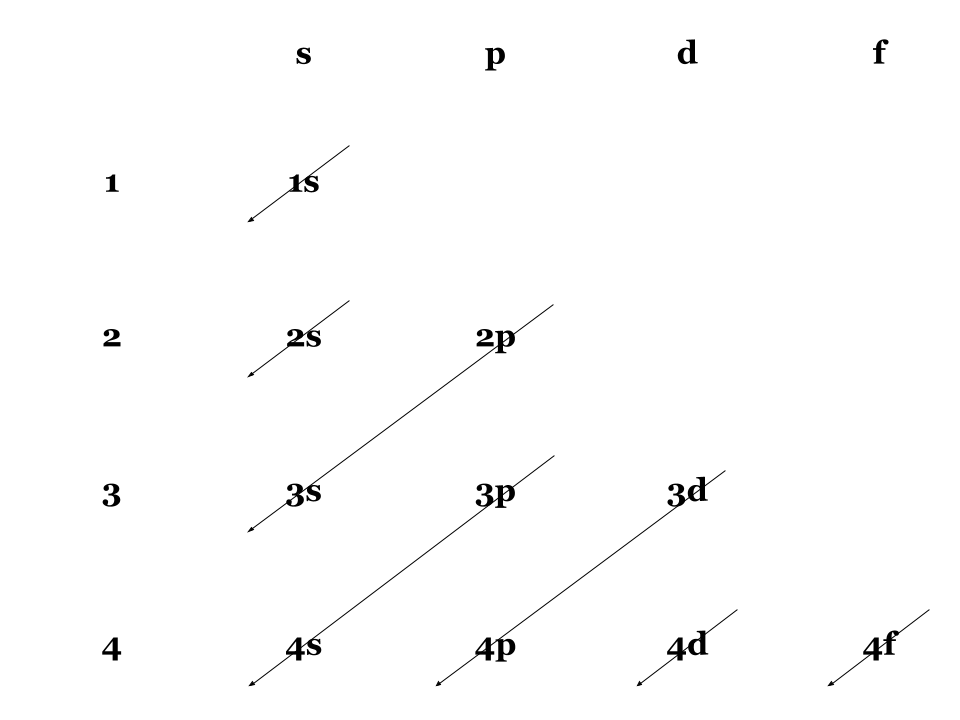
\includegraphics[width = .50\textwidth]{images/electron_config.png}\centering
\end{figure}
 \noindent The $s$ orbital can hold 2 electrons, $p$ can hold 6, $d$ can hold 10, and $f$ can hold 14. Therefore, the ground state electron configuration for phosphorus is

 \begin{gather}
 \boxed{1s^{2} 2s^{2} 2p^{6} 3s^{2} 3d^{3}}\nonumber
 \end{gather}
 \\
 Notice that, for larger electron numbers, $4s$ comes before $3d$.
}



\Problem{18}{A}{%
The key to this problem is to picture this system as a hydrogen-like atom (one electron) with two protons ($Z = 2$). The ionization energy of a hydrogen-like atom can be found using the equation

\begin{gather}
E_{n} = \frac{Z^{2}}{n^{2}} 13.6\Units{eV}
\end{gather}
\\
where $n$ is the state of the system.

\begin{gather}
\therefore \hspace{.1in} E_{1} = Z^{2} \cdot 13.6\Units{eV} = 54.4\Units{eV}\nonumber
\end{gather}
\\
The problem tells us that the energy to remove both electrons from the He atom is $79.0\Units{eV}$. Therefore the energy required to remove one electron is

\begin{gather}
E_{ion} =  79.0\Units{eV} - 54.4\Units{eV} = \boxed{24.6\Units{eV}}\nonumber
\end{gather}
}


\Problem{19}{B}{%
The primary source of the Sun's energy is the Proton-Proton Chain (PP Chain). in this reaction, \textbf{four H\textsuperscript{1}} atoms are fused an eventually create \textbf{one He\textsuperscript{4}} (I say "eventually" because there are 3 reactions in the PP Chain). From the mass-energy equivalence equation and conservation of energy, we know that the energy released during the PP Chain must be the difference in mass between four hydrogen atoms and one helium atom.
}

\Problem{20}{E}{%
This is pure fact recall. Bremsstrahlung refers to the electromagnetic radiation produced by the acceleration or deceleration of a charged particle (usually electrons) after passing through the electric and magnetic fields of a nucleus. This is a smooth, continuous X-ray spectra.
}

\Problem{21}{B}{%
The Rydberg formula for hydrogen is

\begin{gather}
f = \frac{c}{\lambda} = R \left(  \frac{1}{n_{f}^{2}} - \frac{1}{n_{i}^{2}}  \right)
\end{gather}
\\
Where $R$ is The Rydberg Constant and completely unnecessary for the purposes of this problem. Let us say that $\lambda '$ is the wavelength for Lyman-$\alpha$ and $\lambda$ is the wavelength for Balmer-$\alpha$

\begin{align}
\frac{\lambda' }{\lambda} &=  \frac{\left(  \frac{1}{n_{f}^{2}} - \frac{1}{n_{i}^{2}}  \right)}{\left(  \frac{1}{n_{f}'^{2}} - \frac{1}{n_{i}'^{2}}  \right)} = \frac{\left(   \frac{1}{4} - \frac{1}{9}   \right)   }{\left(    \frac{1}{1} -\frac{1}{4}   \right)} = \frac{\left(   \frac{9}{36} - \frac{4}{36}   \right)   }{\left(   \frac{3}{4}   \right)} = \frac{\frac{5}{36}}{\frac{3}{4}} = \frac{20}{108} = \boxed{\frac{5}{27}} \nonumber
\end{align}
\\
Make sure that you dont invert your fraction! Solution (E) is incorrect because it is Balmer-$\alpha$ to Lyman-$\alpha$ radiation and an excellent example of a common GRE a trap answer.
}


\Problem{22}{A}{%
The angular momentum of the moon is the same at every point in it's orbit. The equation for angular momentum, $L$, is

\begin{gather}
L = r \times p = m (r \times v) = m r v \sin{(\theta)}
\end{gather}
\\
The minimum, $r_{p}$, and maximum, $r_{a}$, distances (perigee and apogee) of the orbit correspond to a tangential velocity for which $\theta \hspace{.02in} = \hspace{.03in} 90^{^\circ}$.

\begin{gather}
L = m \cdot v_{a} \cdot r_{a} = m \cdot v_{p} \cdot r_{p}\
\end{gather}
\\
Obviously, we can cancel out the moon's mass, $m$, in the above conservation equation. Therefore we are unable to solve for this mass.\\
\\
Interesting tidbit: when the Soviet Union launched sputnik in 1957, American scientists were unable to determine the satellite's mass for this very reason.
\\\\
}


\Problem{23}{C}{%
The particle is moving with a tangential velocity $v_{\perp} = 10\Units{m/s}$ and the acceleration is $a_{rad} = 10\Units{m/s$^{2}$}$. Since these values have the same magnitude, the angle between the velocity and acceleration vectors is $45^{\circ}$ (picture this as a 45-45-90 triangle).
}

\Problem{24}{C}{%
Gravity only applies in the vertical, $\hat{y}$, direction. Therefore $v_{x}$ is constant with respect to time. This eliminates (A) and (E).\\
\\
Since gravity is working in the $-\hat{y}$ direction while the stone is moving (partly) in the $+\hat{y}$ direction: $v_{y}$ starts positive and decreases with time. At the top of the stone's projectile motion $v_{y} = 0$. Then the stone begins to fall back to the ground so that $v_{y}$ is negative.
}


\Problem{25}{E}{%
The parallel axis theorem is an invaluable tool for computing the moment of inertia of systems built out of smaller pieces whose moments of inertia are known. The moment of inertia about any axis parallel to the center of mass axis is given by the equation

\begin{gather}
\label{eq:par_ax}I = I_{CM} +m r^{2}
\end{gather}
\\
One of these pennies (the middle one) has the same moment of inertia as a disk with radius $r$ and mass $m$. The other 6 require the the parallel axis theorem since the axis of rotation is $2r$ away from each penny's center of mass. The moment of inertia for a disk is $I = \frac{1}{2} m r^{2}$.

\begin{align}
I &= \frac{1}{2} m r^{2} + 6 \left(  \frac{1}{2}mr^2 + m (2r)^{2}  \right) = \frac{1}{2}mr^{2} + 6m r^{2} \left(  \frac{1}{2}  + \frac{8}{2}  \right)  = \boxed{\frac{55}{2} m r^{2}} \nonumber
\end{align}
}

\Problem{26}{C}{%
The moment of inertia for a rod is

\begin{gather}
I = \frac{1}{12} M L^{2}
\end{gather}
\\
We must use the parallel axis theorem (equation \ref{eq:par_ax}) again to to find the moment of inertia about the pivot:

\begin{gather}
I = \frac{1}{12} M L^{2} + M \left(   \frac{L}{2}  \right)^{2} = ML^{2} \left(  \frac{1}{12}  + \frac{3}{12}  \right) = \frac{1}{3}M L^{2}\nonumber
\end{gather}
\\
Now we need to find the speed of the pendulum once the free end hits the ground. The best and easiest way to do this is through use of conservation laws. The free end is $\frac{L}{2}$ above the rod's center of mass and $\omega = \frac{v}{L}$

\begin{align}
m g h &= \frac{1}{2} I \omega^{2}  \nonumber\\
M g \frac{L}{2} &= \frac{1}{2} \left(  \frac{1}{3} M L^{2}  \right) \frac{v^{2}}{L^{2}}   \nonumber\\
gL &= \frac{1}{3}v^{2} \hspace{.1in} \rightarrow \hspace{.1in} \boxed{v = \sqrt{3gL}}  \nonumber
\end{align}
}


\Problem{27}{A}{%
The eigenvalues of a Hermitian operator are always real.\\
\\
Proof: The eigenvalue equation is

\begin{align}
A \ket{\psi} &= \lambda \ket{\psi}\nonumber\\
\therefore \hspace{.1in} A^{\dag} \ket{\psi} &= \lambda^{*} \ket{\psi}\nonumber
\end{align}
\\
Subtracting the second equation from the first we get

\begin{gather}
( A - A^{\dag} )\ket{\psi} = ( \lambda - \lambda^{*} ) \ket{\psi}\nonumber
\end{gather}
The left hand side of the above equation is equal to zero since $A = A^{\dag}$. Therefore, $\lambda = \lambda^{*}$ which means that $\lambda$ is real-valued.
\\\\
}


\Problem{28}{E}{%
Lets say that states n and m are orthonormal: $\braket{ n  | m } = 0$ and $\braket{ n  | n } = \braket{ m  | m } = 1$. Therefore:

\begin{align}
\braket{\psi_{1} | \psi_{2}} &= 0\nonumber\\
&= 5 \braket{ 1 | 1 }  + 15 \braket{ 2 | 2 }  + 2x \braket{ 3 | 3 } \nonumber\\
0 &= 20 + 2x \hspace{.1in} \rightarrow \hspace{.1in} \boxed{x = - 10}\nonumber
\end{align}
\\\\
}

\Problem{29}{C}{%
Recall the Dirac notation identity:

\begin{gather}
\bra{\psi} \hat{A} \ket{\psi} =  \lambda \braket {\psi  | \psi} = \lambda
\end{gather}
\\
Where $\lambda$ is an eigenvalue of $\hat{A}$. From this we can see that, using our given eigenvalues, we get

\begin{align}
\bra{\psi_{-1}} \hat{0} \ket{\psi_{-1}} &= -1 \braket {\psi_{-1}  | \psi_{-1}} = -1\nonumber\\
\bra{\psi_{1}} \hat{0} \ket{\psi_{1}} &= 1 \braket {\psi_{1}  | \psi_{1}} = 1\nonumber\\
\bra{\psi_{2}} \hat{0} \ket{\psi_{2}} &= 2 \braket {\psi_{2}  | \psi_{2}} = 2\nonumber
\end{align}
\\
Therefore,

\begin{gather}
\bra{\psi} \hat{O} \ket{\psi} = \frac{1}{6} \braket {\psi_{-1}  | \psi_{-1}} + \frac{1}{2} \braket {\psi_{1}  | \psi_{1}} + \frac{1}{3} \braket {\psi_{2}  | \psi_{2}} = -\frac{1}{6} + \frac{1}{2} + \frac{2}{3} = \boxed{1}\nonumber
\end{gather}
}


\Problem{30}{A}{%
This kind of problem begs for the process of elimination. Radial wave functions must be normalizable and must go to zero at infinity. Therefore:
\begin{description}
\item[I.] Works. it is normalizable (square integrable) and goes to zero at infinity.
\item[II.] Doesn't work. Sinusoidal functions do not converge and therefore do not go to zero at infinity.
\item[III.] Doesn't work. This function is not normalizable.
\end{description}
}



\end{document}

